\documentclass[tikz,border=12pt]{standalone}
\usepackage[T1]{fontenc}
\usepackage{lmodern}
\usepackage{tikz}
\usetikzlibrary{arrows.meta,calc,positioning}

\definecolor{navy}{HTML}{0C171F}
\definecolor{green}{HTML}{00F700}

\tikzset{
  card/.style={
    draw=navy,
    line width=1.2pt,
    rounded corners=5pt,
    minimum width=4.1cm,
    minimum height=1.8cm,
    align=center,
    text=navy,
    fill=none,
    font=\bfseries\fontsize{15}{18}\selectfont
  },
  flow/.style={
    -{Latex[length=3.4mm,width=2.2mm,fill=green]},
    draw=navy,
    line width=1.4pt
  },
  return/.style={
    flow,
    rounded corners=10pt
  },
  caption/.style={
    text=navy,
    font=\fontsize{10.5}{13}\selectfont
  }
}

\begin{document}
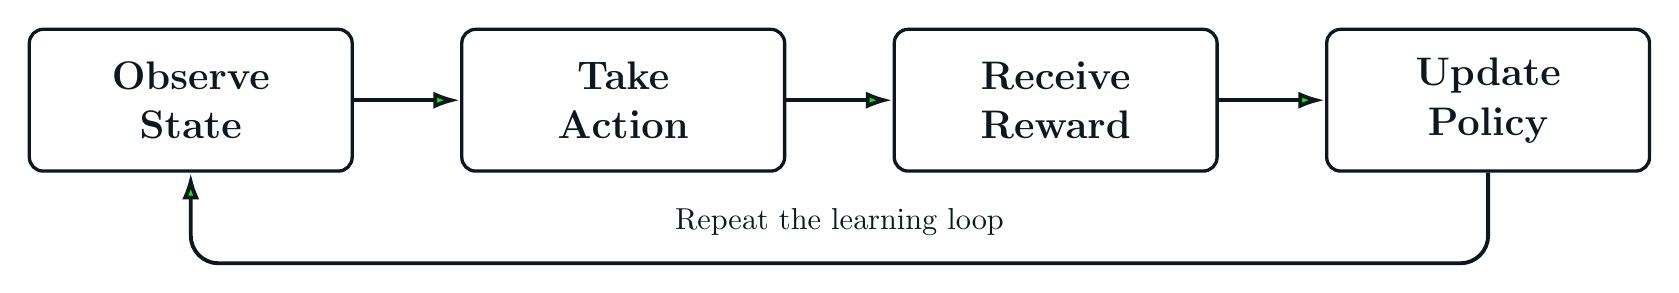
\begin{tikzpicture}
  \node[card] (state) {Observe\\State};
  \node[card, right=1.35cm of state] (action) {Take\\Action};
  \node[card, right=1.35cm of action] (reward) {Receive\\Reward};
  \node[card, right=1.35cm of reward] (update) {Update\\Policy};

  \draw[flow] (state.east) -- (action.west);
  \draw[flow] (action.east) -- (reward.west);
  \draw[flow] (reward.east) -- (update.west);
  \draw[return]
    (update.south) -- ++(0,-1.15cm) -| (state.south);

  \node[caption] at ($(state.south)!0.5!(update.south)+(0,-0.63cm)$)
    {Repeat the learning loop};
\end{tikzpicture}
\end{document}
